\documentclass[12pt, a4paper]{report}

% Packages :

\usepackage[french]{babel}
\usepackage[utf8]{inputenc}
\usepackage[T1]{fontenc}
\usepackage[pdftex, pdfauthor={Bacomathiques}]{hyperref}
\usepackage{sectsty}
\usepackage[explicit]{titlesec}
\usepackage{xcolor}
\usepackage{amsmath}
\usepackage{amssymb}
\usepackage{amsthm}
\usepackage{fourier}
\usepackage{titlesec}
\usepackage{fancyhdr}
\usepackage{catchfilebetweentags}
\usepackage[french, capitalise, noabbrev]{cleveref}
\usepackage[fit, breakall]{truncate}
\usepackage[margin=3cm]{geometry}
\usepackage{tocloft}
\usepackage{tikz}
\usepackage{tocloft}
\usepackage{microtype}
\usepackage{listings}
\usepackage{tabularx}
\usepackage{calc}
\usepackage[export]{adjustbox}
\usepackage[most]{tcolorbox}
\usepackage{standalone}
\usepackage{xlop}
\usepackage{etoolbox}
\usepackage{environ}

\usetikzlibrary{arrows.meta}
\usetikzlibrary{trees}

% Paramètres :

\author{Bacomathiques}
\definecolor{graphe}{HTML}{93c9ff}
\setcounter{MaxMatrixCols}{12}
\setlength{\parindent}{0pt}
\setlength{\fboxsep}{0pt}
%\pdfsuppresswarningpagegroup=1

% Code :

\lstdefinestyle{style}{
	backgroundcolor=\color{white},
	commentstyle=\em\color[HTML]{999988},
	keywordstyle=\bfseries,
	identifierstyle=\normalfont,
	stringstyle=\color[rgb]{0.87, 0.07, 0.27},
	basicstyle=\ttfamily\color{black},
	breakatwhitespace=false,
	breaklines=true,
	captionpos=b,
	keepspaces=true,
	numbers=left,
	numbersep=5pt,
	showspaces=false,
	showstringspaces=false,
	showtabs=false,
	tabsize=2,
	numbers=none
}

\lstset{style=style}
\lstset{
	literate=
	{á}{{\'a}}1
	{à}{{\`a}}1
	{ã}{{\~a}}1
	{é}{{\'e}}1
	{ê}{{\^e}}1
	{í}{{\'i}}1
	{ó}{{\'o}}1
	{õ}{{\~o}}1
	{ú}{{\'u}}1
	{ü}{{\"u}}1
	{ç}{{\c{c}}}1
}

\lstset{
	framextopmargin=10pt,
	framexrightmargin=10pt,
	framexbottommargin=10pt,
	framexleftmargin=10pt,
	xleftmargin=10pt,
	xrightmargin=10pt,
}

% Couleurs :

\definecolor{title}{HTML}{912c21}
\definecolor{section}{HTML}{1c567d}
\definecolor{subsection}{HTML}{2980b9}

\definecolor{rule}{HTML}{c4c4c4}

\definecolor{formula}{HTML}{ebf3fb}
\definecolor{formula-left}{HTML}{3583d6}

\definecolor{tip}{HTML}{dcf3d8}
\definecolor{tip-left}{HTML}{26a65b}

\definecolor{demonstration}{HTML}{fff8de}
\definecolor{demonstration-left}{HTML}{f1c40f}

\definecolor{exercise}{HTML}{e0f2f1}
\definecolor{exercise-left}{HTML}{009688}

\definecolor{correction}{HTML}{e0f7fa}
\definecolor{correction-left}{HTML}{00bcd4}

\definecolor{toc}{HTML}{fceae9}
\definecolor{toc-left}{HTML}{e74c3c}
\definecolor{toc-dark}{HTML}{87281f}

% Titres :

\renewcommand{\thesection}{\Roman{section} - }
\renewcommand{\thesubsection}{\arabic{subsection}. }

\newcommand{\sectionstyle}{\normalfont\LARGE\bfseries\color{section}}
\titleformat{\section}{\sectionstyle}{\thesection #1}{0pt}{}
\titleformat{name=\section, numberless}{\sectionstyle}{#1}{0pt}{}

\newcommand{\subsectionstyle}{\normalfont\Large\bfseries\color{subsection}}
\titleformat{\subsection}{\subsectionstyle}{\thesubsection #1}{0pt}{}
\titleformat{name=\subsection, numberless}{\subsectionstyle}{#1}{0pt}{}

\titlelabel{\thetitle\ }

% Table des matières :

\addto\captionsfrench{\renewcommand\contentsname{}}
\renewcommand{\cftsecpagefont}{\color{toc-dark}}
\renewcommand{\cftsubsecpagefont}{\color{toc-dark}}
\renewcommand{\cftsecleader}{\cftdotfill{\cftdotsep}}
\renewcommand{\cftsecfont}{\bfseries}
\renewcommand{\cftsecpagefont}{\bfseries\color{toc-dark}}
\setlength{\cftbeforetoctitleskip}{0pt}
\setlength{\cftaftertoctitleskip}{0pt}
\setlength{\cftsecindent}{0pt}
\setlength{\cftsubsecindent}{20pt}
\setlength{\cftsubsecnumwidth}{20pt}

% Commandes :

\newcommand{\newpar}{\\[\medskipamount]}
\newcommand{\lesson}[3]{%
	\newcommand{\level}{#1}%
	\newcommand{\id}{#2}%
	\hypersetup{pdftitle={#3}}
	\begin{center}%
		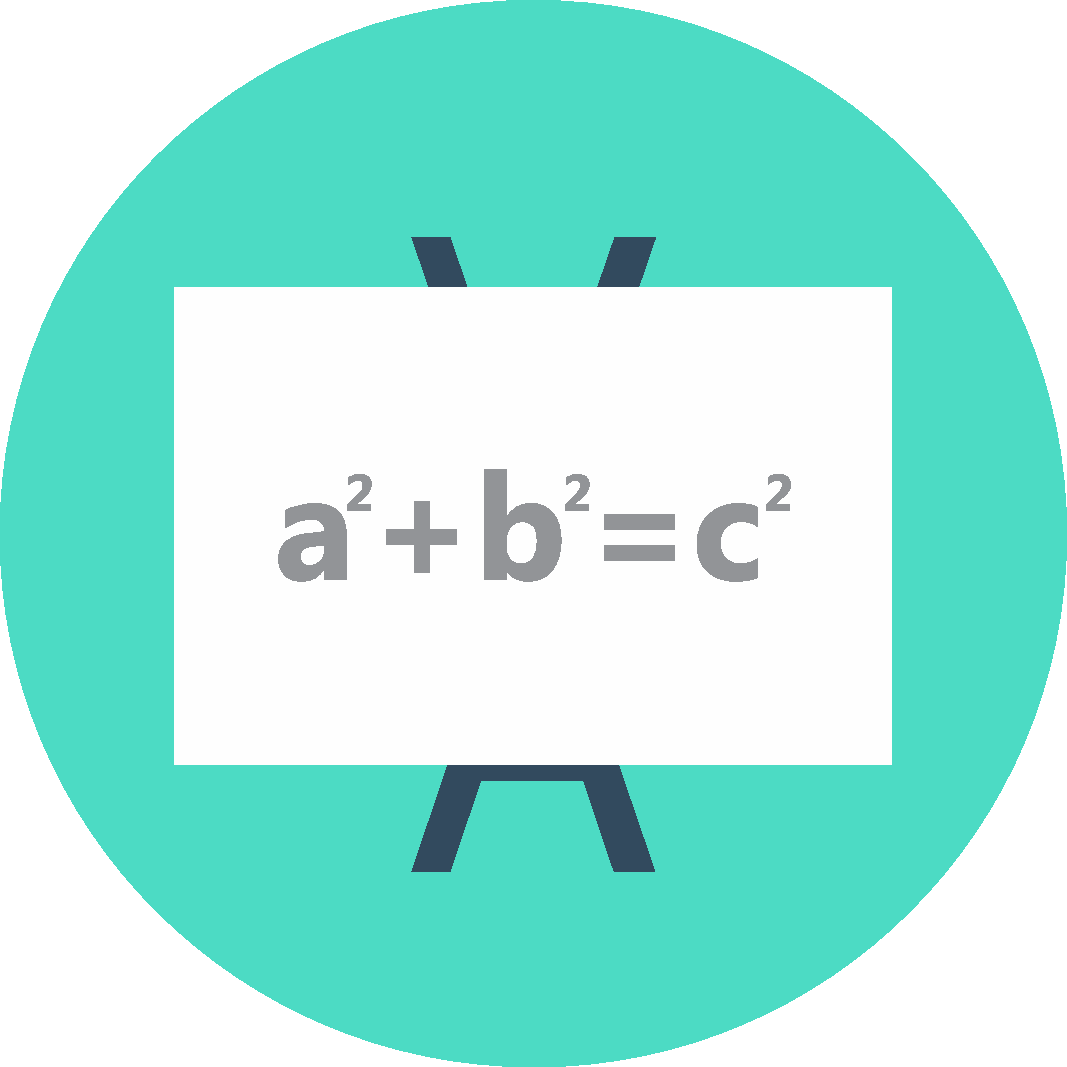
\includegraphics[width=150px]{\imagespath/bacomathiques}%
		
		\vspace{30pt}%
		{\Huge\color{title} #3}%
		
		\vspace{10pt}%
		{Bacomathiques --- \href{https://bacomathiqu.es/cours/#1/#2}{\color{section} https://bacomathiqu.es}}%
		
		\vspace{20pt}%
	\end{center}%
	\begin{toc}
		\tableofcontents%
	\end{toc}
	\thispagestyle{empty}%
	\newpage%
	\setcounter{page}{1}%
}
\newcommand{\imagespath}{../../images}
\newcommand{\lessonimagespath}{\imagespath/lessons/\level/\id/}
\newcommand{\includelatexpicture}[2][\textwidth - 100pt]{%
	\begin{center}%
		\resizebox{#1}{!}{%
			\input{\lessonimagespath#2}%
		}%
	\end{center}%
	\medskip%
}
\newcommand{\includeimage}[1]{%
	\begin{center}%
		\includegraphics{\lessonimagespath#1}%
	\end{center}%
	\medskip%
}
\newcommand{\includerepresentation}[1]{%
	\begin{center}%
		\setlength{\fboxrule}{0.5pt}%
		\href{https://www.geogebra.org/m/#1}{\includegraphics[width=\textwidth-1pt,fbox]{\lessonimagespath#1}}%
	\end{center}%
}
\newcommand{\floor}[1]{\lfloor #1 \rfloor}

\makeatletter
\newcommand\inputcontent{\@ifstar{\inputcontent@star}{\inputcontent@nostar}}
\newcommand{\inputcontent@star}[1]{%
	\ExecuteMetaData[#1]{content}%
}
\newcommand{\inputcontent@nostar}[1]{%
	\newpage%
	\inputcontent@star{#1}%
}
\makeatother

\let\oldsection\section
\renewcommand\section{\clearpage\oldsection}
\newcommand{\contentwidth}[1][medium]{}

% En-têtes :

\pagestyle{fancy}

\renewcommand{\sectionmark}[1]{\markboth{\thesection \ #1}{}}

\fancyhead[R]{\truncate{0.23\textwidth}{\color{title}\thepage}}
\fancyhead[L]{\truncate{0.73\textwidth}{\color{title}\leftmark}}
\fancyfoot[C]{\scriptsize \href{https://bacomathiqu.es/cours/\level/\id}{\texttt{bacomathiqu.es}}}

\makeatletter
\patchcmd{\f@nch@head}{\rlap}{\color{rule}\rlap}{}{}
\patchcmd{\headrule}{\hrule}{\color{rule}\hrule}{}{}
\makeatother

% Environnements :

\newenvironment{nosummary}{}{}
\newcommand{\tcolorboxtitle}[2]{\setlength{\fboxsep}{2.5pt}\hspace{-10pt}\colorbox{#1-left}{\hspace{8pt}\MakeUppercase{#2} \hspace{2pt} \includegraphics[height=0.8em]{\imagespath/bubbles/#1}\hspace{5pt}}}
\newcommand{\tcolorboxsubtitle}[2]{\ifstrempty{#2}{}{\textcolor{#1-left}{\large#2}\\[\medskipamount]}}
\tcbset{
	frame hidden,
	boxrule=0pt,
	boxsep=0pt,
	enlarge bottom by=8.5pt,
	enhanced jigsaw,
	boxed title style={sharp corners,boxrule=0pt,coltitle={white},titlerule=0pt},
	fonttitle=\fontsize{6pt}{6pt}\bfseries\boldmath,
	top=10pt,
	right=10pt,
	bottom=10pt,
	left=10pt,
	arc=0pt,
	outer arc=0pt,
}
\newtcolorbox{toc}[1][]{
	colback=toc,
	borderline west={3pt}{0pt}{toc-left},
	title=\tcolorboxtitle{toc}{Table des matières},
	colbacktitle=toc,
	before upper={\tcolorboxsubtitle{toc}{#1}}
}
\newtcolorbox{formula}[1][]{
	colback=formula,
	borderline west={3pt}{0pt}{formula-left},
	title=\tcolorboxtitle{formula}{À retenir},
	colbacktitle=formula,
	before upper={\tcolorboxsubtitle{formula}{#1}}
}
\newtcolorbox{tip}[1][]{
	colback=tip,
	borderline west={3pt}{0pt}{tip-left},
	title=\tcolorboxtitle{tip}{À lire},
	colbacktitle=tip,
	before upper={\tcolorboxsubtitle{tip}{#1}}
}
\newtcolorbox{demonstration}[1][]{
	colback=demonstration,
	borderline west={3pt}{0pt}{demonstration-left},
	title=\tcolorboxtitle{demonstration}{Démonstration},
	colbacktitle=demonstration,
	before upper={\tcolorboxsubtitle{demonstration}{#1}}
}

\NewEnviron{whitetabularx}[1]{%
	\renewcommand{\arraystretch}{2.5}
	\colorbox{white}{%
		\begin{tabularx}{\textwidth}{#1}%
			\BODY%
		\end{tabularx}%
	}%
}

% Longueurs :

\newlength{\espacetitreliste}
\setlength{\espacetitreliste}{-16pt}
\newcommand{\entretitreetliste}{\vspace{\espacetitreliste}}

\begin{document}
	%<*content>
	\lesson{premiere}{suites}{Chapitre I – Les suites}
	
	\section{Généralités}
	
	\subsection{Définition}
	
	On appelle \textbf{suite} une fonction de $\mathbb{N}$ dans $\mathbb{R}$ : cette fonction va prendre des éléments de l'ensemble de départ $\mathbb{N}$ et va les amener dans l'ensemble d'arrivée $\mathbb{R}$.
	
	\begin{formula}[Définition]
		Il y a plusieurs manières de définir une suite :
		\begin{itemize}
			\item \textbf{Par récurrence :} On donne le premier terme de la suite ainsi que le terme au rang $n+1$.
			\item \textbf{Par son terme général :} On donne le $n$-ième terme de la suite en fonction de $n$.
		\end{itemize}
	\end{formula}
	
	\textbf{Attention !} Bien que ces deux modes de génération soient les principaux, il en existe d'autres : algorithme, motifs géométriques, ...
	
	\begin{tip}[Exemple]
		On définit les suites $(u_n)$ et $(v_n)$ ainsi :
		\begin{itemize}
			\item $u_n = n$ pour tout $n \in \mathbb{N}$ ($(u_n)$ est définie par son terme général).
			\item $(v_n) = \begin{cases} v_0 = 0 \\ v_{n+1} = v_n + 1 \text{ pour tout } n \geq 1 \end{cases}$ ($(v_n)$ est définie par récurrence).
		\end{itemize}
		On remarque que bien que définies différemment, $(u_n)$ et $(v_n)$ sont égales.
	\end{tip}
	
	\begin{tip}
		À ne pas confondre :
		\begin{itemize}
			\item $(u_n)$ qui est la \textbf{suite} $(u_n)$.
			\item $u_n$ qui est le \textbf{$n$-ième terme} de la suite $(u_n)$.
		\end{itemize}
		Ce ne sont pas les mêmes objets : le premier est une suite, le second est un réel.
	\end{tip}
	
	\subsection{Suites arithmétiques}
	
	\begin{formula}[Définition]
		Une suite $(u_n)$ est dite \textbf{arithmétique} si elle est de la forme $u_{n+1} = u_n + r$ avec $r \in \mathbb{R}$.
	\end{formula}
	
	\begin{formula}[Raison]
		Le réel $r$ est la \textbf{raison} de la suite (si $r > 0$, $(u_n)$ est strictement croissante, si $r < 0$, $(u_n)$ est strictement décroissante et si $r = 0$, $(u_n)$ est constante).
	\end{formula}
	
	Il est possible de trouver le terme général d'une suite arithmétique :
	
	\begin{formula}[Terme général]
		On note $p$ le rang initial de la suite (celui à partir duquel la suite est définie) :
		\newpar
		$u_n = u_p + (n-p) \times r$
		\newpar
		Et si $(u_n)$ est définie à partir du rang $0$ (on a $p = 0$) :
		\newpar
		$u_n = u_0 + (n-0) \times r = u_0 + n \times r$
	\end{formula}
	
	\begin{demonstration}[Terme général]
		On a $u_{p+1} = u_p + r$. Puis, $u_{p+2} = u_{p+1} + r = u_p + r + r = u_p + 2 \times r$. De même, $u_{p+3} = u_{p+2} + r = u_p + 3 \times r$  et caetera.
		\newline
		En fait, pour tout $k$ entier plus grand que $p$, on a $u_{p+k} = u_p + k \times r$.
		\newline
		Donc si on pose $n = p+k$, alors $u_n = u_p + (n-p) \times r$.
	\end{demonstration}
	
	\begin{formula}[Somme des termes]
		$\displaystyle{1 + 2 + \dots + n = \frac{n(n + 1)}{2}}$ pour tout $n \in \mathbb{N}$.
	\end{formula}
	
	\begin{demonstration}[Somme des termes]
		On pose pour tout $n \in \mathbb{N}$, $S_n = 1 + 2 + \dots + n$. On a également $S_n = n + (n-1) + \dots + 1$ (en écrivant la somme à l'envers).
		\newline
		D'où $S_n + S_n = 2S_n = \underbrace{(n + 1) + (n + 1) + \dots + (n + 1)}_{n \text{ fois}} = n \times (n + 1)$. Et ainsi $\displaystyle{S_n = \frac{n(n + 1)}{2}}$.
	\end{demonstration}
	
	\begin{tip}[Exemple]
		On souhaite calculer $S = 24 + 25 + \dots + 104$.
		\newpar
		En fait, $S = 1 + 2 + \dots + 23 + 24 + 25 + \dots + 104 - (1 + 2 + \dots + 23)$. Calculons les deux sommes séparément :
		\begin{itemize}
			\item $1 + 2 + \dots + 23 = \displaystyle{\frac{23 \times 24}{2}} = 276$
			\item $1 + 2 + \dots + 104 = \displaystyle{\frac{104 \times 105}{2}} = 5460$
		\end{itemize}
		D'où $S = 5460 - 276 = 5184$.
	\end{tip}
	
	\subsection{Suites géométriques}
	
	\begin{formula}[Définition]
		Une suite $(v_n)$ est dite \textbf{géométrique} si elle est de la forme $v_{n+1} = v_n \times q$ avec $q \in \mathbb{R}$.
	\end{formula}
	
	\begin{formula}[Raison]
		Le réel $q$ est la \textbf{raison} de la suite (si $q > 1$, $(v_n)$ est strictement croissante, si $0 < q < 1$, $(v_n)$ est strictement décroissante et si $q = 1$ ou $0$, $(v_n)$ est constante).
	\end{formula}
	
	Il est possible de trouver le terme général d'une suite géométrique :
	
	\begin{formula}[Terme général]
		On note $p$ le rang initial de la suite (celui à partir duquel la suite est définie) :
		\newpar
		$v_n = v_p \times q^{n-p}$
		\newpar
		Et si $(v_n)$ est définie à partir du rang $0$ (on a $p = 0$) :
		\newpar
		$v_n = v_0 \times q^{n-0} = v_0 \times q^n$
	\end{formula}
	
	\begin{demonstration}[Terme général]
		On a $v_{p+1} = v_p \times q$. Puis, $v_{p+2} = v_{p+1} \times q = v_p \times q \times q = v_p \times q^2$. De même, $v_{p+3} = v_{p+2} \times q = v_p \times q^3$  et caetera.
		\newline
		En fait, pour tout $k$ entier plus grand que $p$, on a $v_{p+k} = v_p \times q^k$.
		\newline
		Donc si on pose $n = p+k$, alors $v_n = v_p \times q^{n-p}$.
	\end{demonstration}
	
	\begin{formula}[Somme des termes]
		Soit $n \neq 0$ un entier et $q$ un réel, alors :
		\begin{itemize}
			\item Si $q \neq 1$, alors $\displaystyle{1 + q^1 + q^2 + \dots + q^n = \frac{1 - q^{n + 1}}{1 - q}}$.
			\item Si $q = 1$, alors $\displaystyle{1 + q^1 + q^2 + \dots + q^n = \underbrace{1 + 1 + 1 + \dots + 1}_{n \text{ fois}} = n}$.
		\end{itemize}
	\end{formula}
	
	\begin{demonstration}[Somme des termes]
		Le cas $q = 1$ étant donné juste au-dessus, on supposera $q \neq 1$. On pose pour tout $n \in \mathbb{N}$, $S_n = 1 + q^1 + q^2 + \dots + q^n$.
		\newpar
		On a : $qS_n = q^1 + q^2 + q^3 + \dots + q^{n+1}$, puis : $S_n - qS_n = 1 + q^1 + q^2 + \dots + q^n - q^1 - q^2 - q^3 - \dots - q^{n+1} = 1 - q^{n+1}$.
		\newpar
		Donc on a en factorisant par $S_n$ : $(1 - q)S_n = 1 - q^{n+1} \iff S_n = \frac{1 - q^{n+1}}{1 - q}$.
		\newpar
	\end{demonstration}
	
	\begin{tip}[Exemple]
		On souhaite calculer $S = 3^5 + 3^6 + \dots + 3^{10}$.
		\newpar
		En fait, $S = 1 + 3 + \dots + 3^4 + 3^5 + 3^6 + \dots + 3^{10} - (1 + \dots + 3^4)$. Calculons les deux sommes séparément :
		\begin{itemize}
			\item $1 + 3 + \dots + 3^4 = \displaystyle{\frac{1 - 3^5}{1 - 3}} = 121$
			\item $1 + 3 + \dots + 3^{10} = \displaystyle{\frac{1 - 3^{11}}{1 - 3}} = 88573$
		\end{itemize}
		D'où $S = 88573 - 121 = 88452$.
	\end{tip}
	
	\section{Étude des suites}
	
	\subsection{Sens de variation}
	
	\begin{formula}[Définition]
		Soit $(u_n)$ une suite.
		\begin{itemize}
			\item $(u_n)$ est \textbf{croissante} si on a $u_{n+1} \geq u_n$ (ou $u_{n+1} - u_n \geq 0$) pour tout $n \in \mathbb{N}$.
			\item $(u_n)$ est \textbf{décroissante} si on a $u_{n+1} \leq u_n$ (ou $u_{n+1} - u_n \leq 0$) pour tout $n \in \mathbb{N}$.
			\item $(u_n)$ est dite \textbf{constante} s'il existe $c \in \mathbb{R}$ tel que $u_n = c$ pour tout $n \in \mathbb{N}$.
		\end{itemize}
	\end{formula}
	
	Si une suite est croissante ou décroissante et ne change pas de variation, alors elle est dite \textbf{monotone}.
	
	\subsection{Introduction aux limites}
	
	Quand on souhaite s'intéresser à la limite d'une suite $(u_n)$, on étudie le comportement de ses termes quand``$n$ devient très grand''. On préfère dire alors que \textbf{$n$ tend vers $+\infty$}.
	
	\begin{formula}[Définition]
		Soit $(u_n)$ une suite.
		\begin{itemize}
			\item Si $(u_n)$ tend vers un réel quand $n$ tend vers $+\infty$, on dit qu'elle \textbf{converge}.
			\item Si $(u_n)$ tend vers une limite infinie quand $n$ tend vers $+\infty$, on dit qu'elle \textbf{diverge}.
		\end{itemize}
	\end{formula}
	
	\begin{tip}[Exemple]
		On définit la suite $(u_n)$ pour tout $n \in \mathbb{N}$ par $u_n = \frac{1}{n}$. On souhaite trouver la limite possible de cette suite en $+ \infty$.
		\newline
		Pour cela, regardons les valeurs que prend cette suite pour des valeurs de $n$ très grandes :
		\newpar
		\begin{whitetabularx}{|X|X|}
			\hline
			$100$ & $0,01$ \\
			\hline
			$1 000$ & $0,001$ \\
			\hline
			$100 000$ & $0,000 01$ \\
			\hline
			$1 000 000 000$ & $0,000 000 001$ \\
			\hline
		\end{whitetabularx}
		\newpar
		\textbf{Il semble que} cette suite converge vers 0.
	\end{tip}
	
	À savoir que si une suite a une limite, alors cette limite est \textbf{unique}. Mais il est également possible pour une suite de ne pas admettre de limite.
	
	\begin{tip}[Exemple]
		On définit la suite $(u_n)$ pour tout $n \in \mathbb{N}$ par $u_n = (-1)^n$. On souhaite trouver la limite possible de cette suite en $+ \infty$.
		\newpar
		\begin{whitetabularx}{|X|X|}
			\hline
			$100$ & $1$ \\
			\hline
			$101$ & $-1$ \\
			\hline
			$1 000 000$ & $1$ \\
			\hline
			$1 000 001$ & $-1$ \\
			\hline
		\end{whitetabularx}
		\newpar
		En fait, si $n$ est pair cette suite vaut $1$ et si $n$ est impair elle vaut $-1$. Cette suite n'admet donc pas de limite : elle diverge.
	\end{tip}
	
	\subsection{Représentation graphique}
	
	Il est possible de représenter graphiquement une suite. Cela peut aider, par exemple dans le but de chercher sa limite.
	
	\begin{formula}[Méthode pour une suite définie par récurrence]
		Soit $(u_n)$ une suite définie par récurrence. Pour représenter $(u_n)$ dans un graphique :
		\begin{enumerate}
			\item On trace la droite d'équation $y = x$.
			\item  Comme cette suite est définie par récurrence, pour tout entier $n$ on a une relation du type $u_{n+1} = f(u_n)$. Il s'agit de tracer la courbe représentative $\mathcal{C}_f$ de la fonction $f$.
			\item On place le point $A$ de coordonnées $(u_0; 0)$
			\item On trace une droite verticale passant par $A$, son intersection avec $\mathcal{C}_f$ donne un point $B = (u_0; u_1)$.
			\item À l'aide du point $B$, on place le point $C = (0; u_1)$.
			\item On trace une droite horizontale passant par $C$, son intersection avec la droite $y = x$ donne un point $D = (u_1; u_1)$.
			\item Une fois le point $D$ obtenu, on place le point $(u_1; 0)$.
			\item On recommence l'opération en remplaçant $u_0$ par $u_1$ et $u_1$ par $u_2$, puis on recommence, etc.
		\end{enumerate}
	\end{formula}
	
	\begin{tip}[Exemple]
		Représentation des trois premiers termes de la suite $(u_n) = \begin{cases} u_0 = 3 \\ u_{n+1} = \frac{u_n}{2} \end{cases}$.
		\includerepresentation{zkvhccnn}
	\end{tip}
	
	Il est cependant plus facile de représenter graphiquement une suite dont on connaît le terme général.
	
	\begin{formula}[Méthode pour une suite définie par son terme général]
		Soit $(v_n)$ une suite définie par son terme général. Pour représenter $(v_n)$ dans un graphique :
		\begin{enumerate}
			\item On place le point de coordonnées $(0; v_0)$.
			\item On place le point de coordonnées $(1; v_1)$.
			\item On place le point de coordonnées $(2; v_2)$. Etc.
		\end{enumerate}
	\end{formula}
	
	\begin{tip}[Exemple]
		Représentation des trois premiers termes de la suite $(v_n)$ définie pour tout $n \in \mathbb{N}$ par $v_n = 2^n$.
		\includerepresentation{qvc3drk9}
	\end{tip}
	%</content>
\end{document}